\chapter{Результаты}
\label{chapter_results}

В данной главе приводятся результаты тестирования разработанных методов адаптивного выбора параметров ЭА на модельных задачах. В качестве модельных задач использовались известные задачи числовой оптимизации, решаемые с помощью $(\mu + \lambda)$-эволюционной стратегии. Приводятся результаты сравнения существующих методов с существующими методами настройки параметров ЭА с помощью обучения с подкреплением. Также исследуется эффективность существующих методов выделения состояний среды.

В качестве особи рассматривался набор вещественных чисел $x_1, \ldots, x_n$ -- текущее решение задачи оптимизации, где $n$ -- размерность решаемой задачи. В качестве эволюционных операторов применялся только оператор мутации, определяемый следующим образом:
\begin{equation}
 \begin{pmatrix} x_1 \\ .. \\ x_n \end{pmatrix} = \begin{pmatrix} x_1 \\ .. \\ x_n \end{pmatrix} + \sigma \begin{pmatrix}dx_1 \\ .. \\ dx_n\end{pmatrix}, 
\end{equation}
где $dx_i \sim \mathcal{N}(0, 1)$, а $\sigma$ -- настраиваемый параметр, называемый \textit{шагом}. Значения параметра $\sigma$ лежат в некотором диапазоне $[0, k]$, где $k$ -- некоторая константа. В рамках данной работы проводились эксперименты с различными значениями параметра $k$. Ожидаемым поведением методов адаптивного выбора параметров ЭА является уменьшение значения шага мутации при приближении к оптальному решению. 

Далее подробно описываются модельные задачи, на которых проводилось экспериментальное исследование методов настройки параметров ЭА. Для каждой задачи приводятся результаты ее решения. 
 
\section{Сфера}

Необходимо с точностью $\epsilon$ найти минимум унимодальной сферической функции~(\ref{sphere_eq}).
\begin{equation}
\label{sphere_eq}
f(x_1,..,x_n) = \sum\limits_{i=1}^n{x_i^2}
\end{equation}
График функции для двух переменных представлен на рис.~\ref{sphere_plot}. При $x_i \in [-10; 15]$ глобальный минимум достигается в точке $(0,..,0)$.

\begin{figure}
    \centering
    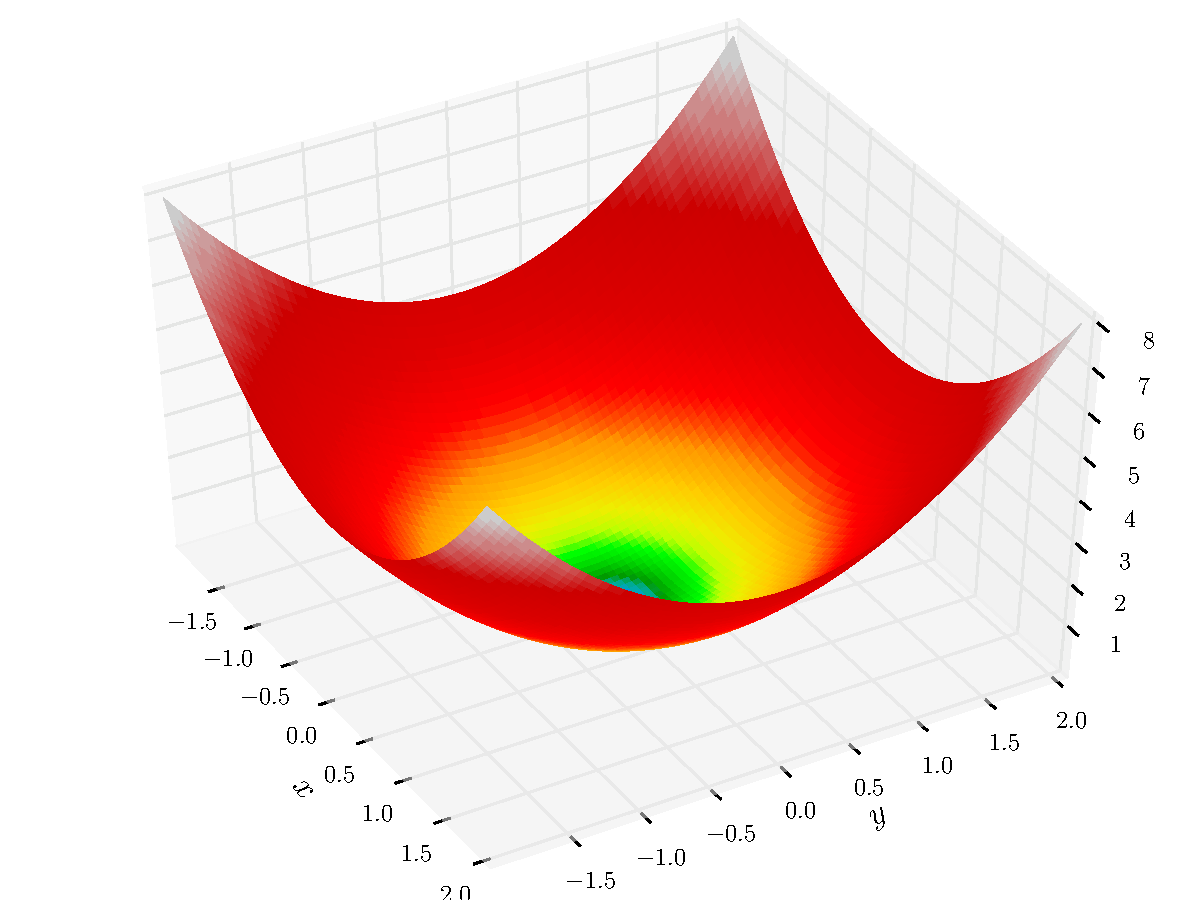
\includegraphics[width=0.6\textwidth]{sphere.pdf}
    \caption{График сферической функции для двух переменных.}
    \label{sphere_plot}
\end{figure}

\begin{figure}
    \centering
    \label{earpc_sphere_dist}
    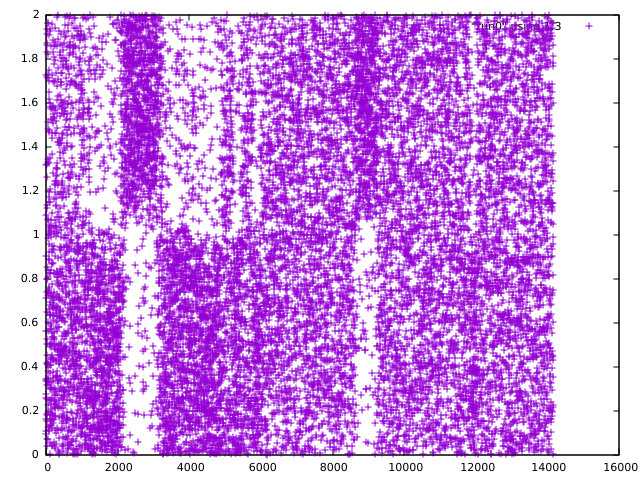
\includegraphics[width=0.6\textwidth]{earpc_sphere_dist.png}
    \caption{График выбранных значений $\sigma$ с помощью метода \textit{earpc}}
\end{figure}


\begin{figure}
\label{earpc_sphere}
    \centering
    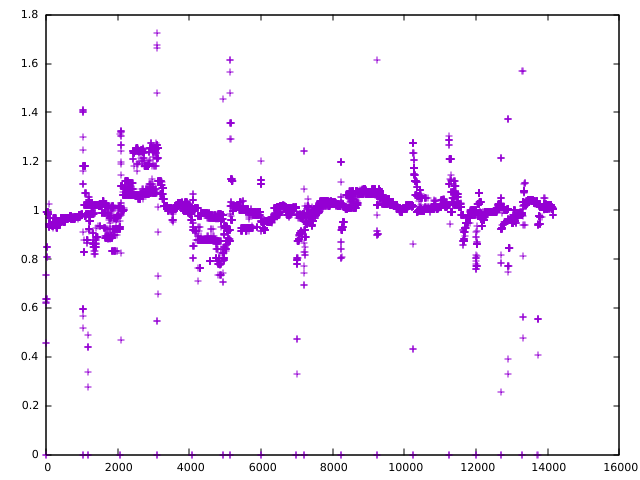
\includegraphics[width=0.6\textwidth]{earpc_sphere.png}
    \caption{График точки разбиения в методе \textit{earpc}}
\end{figure}

\begin{figure}
\label{dist_sphere}
    \centering
    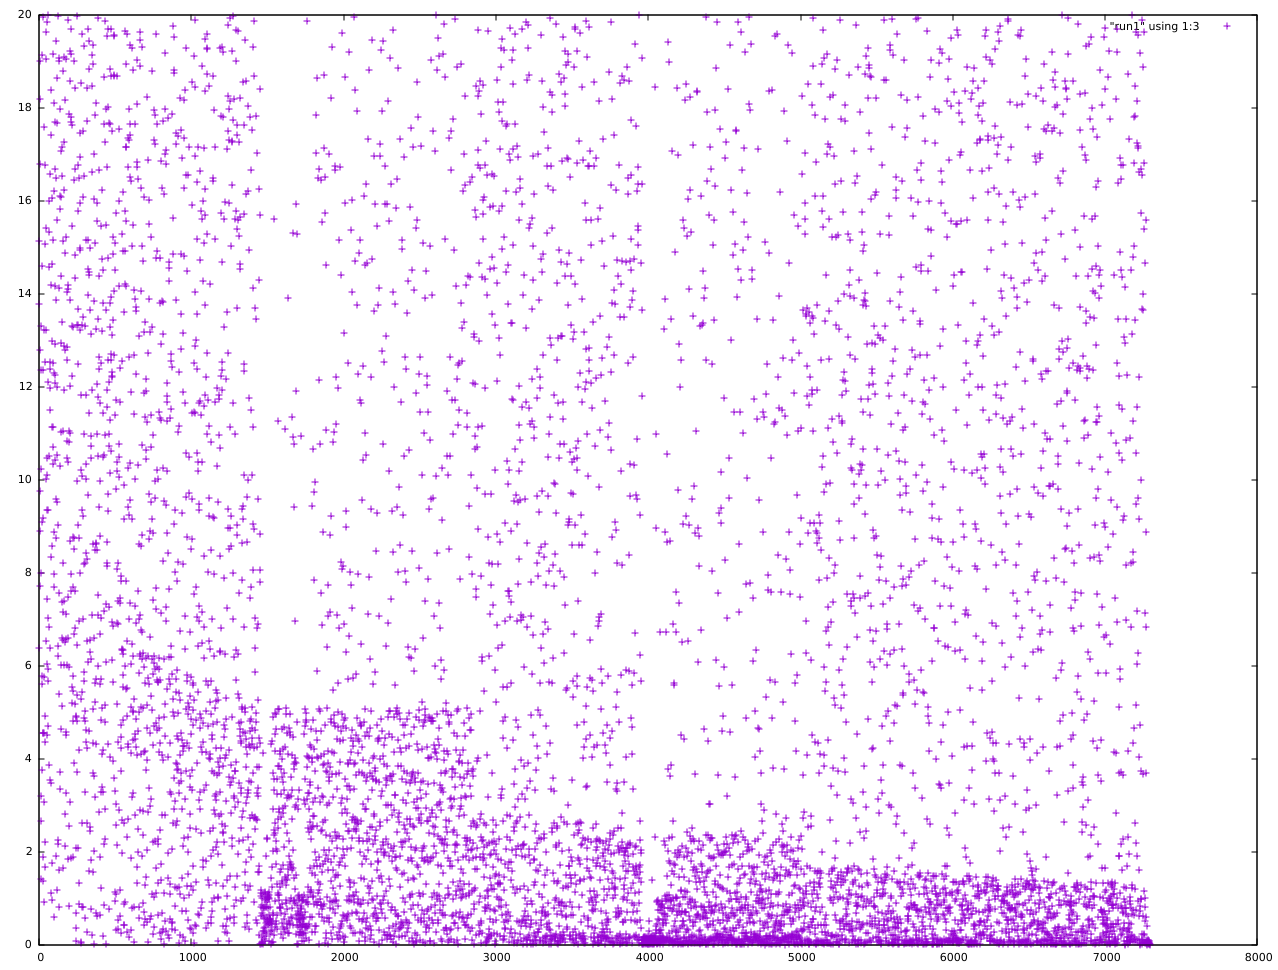
\includegraphics[width=0.6\textwidth]{dist_sphere_dist.png}
    \caption{График выбранных значений $\sigma$ с помощью предложенного метода}
\end{figure}

\begin{figure}
    \centering
    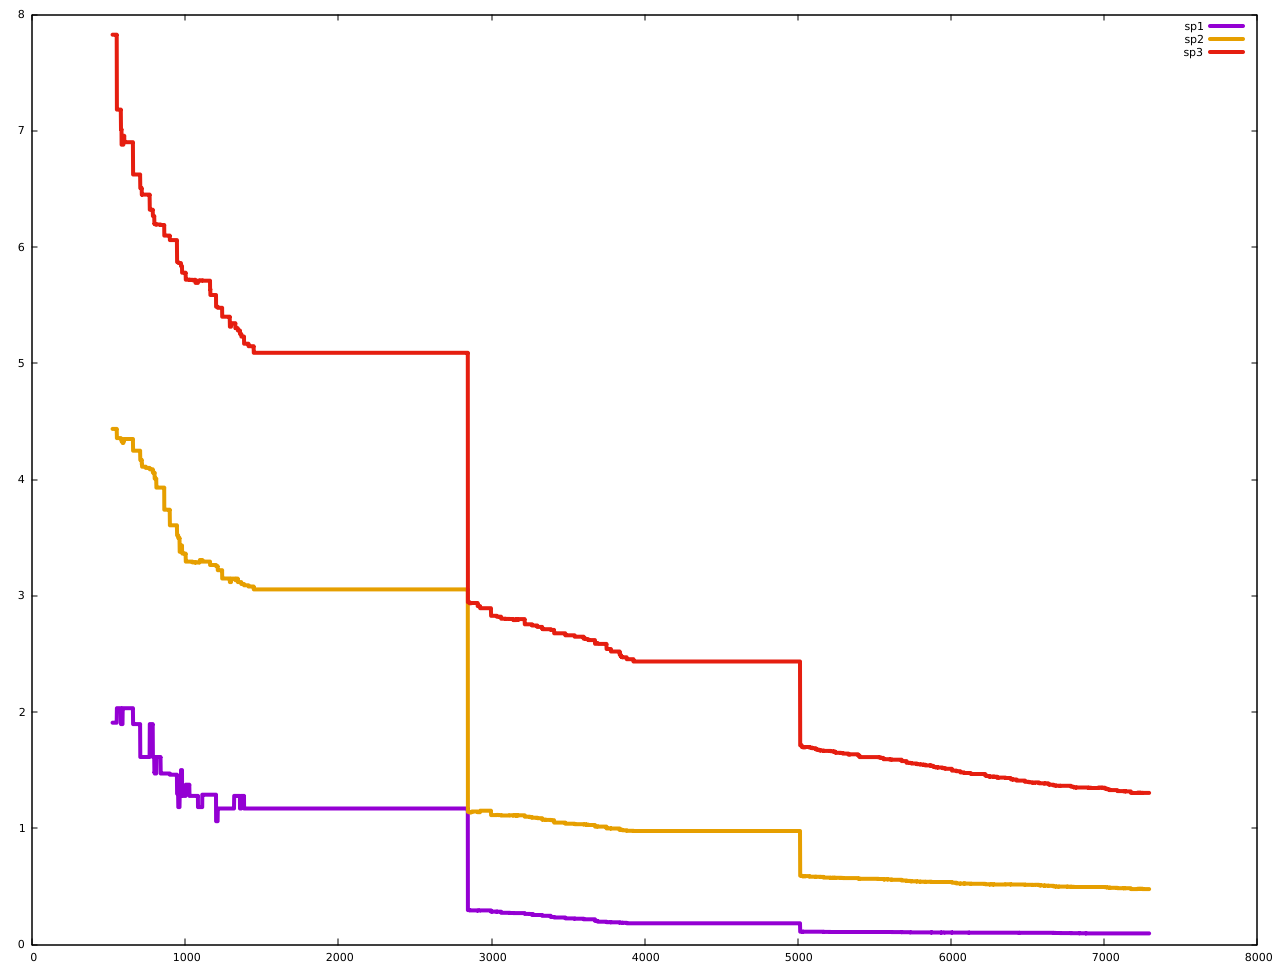
\includegraphics[width=0.6\textwidth]{dist_sphere.png}
    \caption{График точек разбиения в предложенном методе}
\end{figure}


\begin{table}
\label{sphere_results}
  \centering
\begin{tabular}{|*4{c|}}
\hline
\multicolumn{4}{|l|}{k = 1} \\
\hline
\diagbox{$\mu$}{$\lambda$} & \multicolumn{1}{c|}{1} & \multicolumn{1}{c|}{3} & \multicolumn{1}{c|}{7} \\
\hline
1 & 4830 & 2462 & 878 \\
\hline
5 & 1450 & 695 & 368 \\
\hline
10 & 808 & 551 & 218 \\
\hline
\multicolumn{4}{|l|}{k = 2} \\
\hline
\diagbox{$\mu$}{$\lambda$} & \multicolumn{1}{c|}{1} & \multicolumn{1}{c|}{3} & \multicolumn{1}{c|}{7} \\
\hline
1 & 4342 & 2333 & 1464 \\
\hline
5 & 1891 & 974 & 695 \\
\hline
10 & 1164 & 672 & 509 \\
\hline
\multicolumn{4}{|l|}{k = 3} \\
\hline
\diagbox{$\mu$}{$\lambda$} & \multicolumn{1}{c|}{1} & \multicolumn{1}{c|}{3} & \multicolumn{1}{c|}{7} \\
\hline
1 & 8199 & 2826 & 1427 \\
\hline
5 & 2447 & 1445 & 910 \\
\hline
10 & 1996 & 1152 & 653 \\
\hline
\end{tabular}
  \captionsetup{justification=centering}
    \caption{Таблица с результатами}
\end{table}

\begin{table}
\begin{tabular}{|*7{c|}}
\hline
\multicolumn{7}{|l|}{k = 1} \\
\hline
\multirow{2}{*}{\diagbox{$\mu$}{$\lambda$}} & \multicolumn{2}{c|}{1} & \multicolumn{2}{c|}{3} & \multicolumn{2}{c|}{7} \\
\cline{2-7}
 & q-learn & gecco & q-learn & gecco & q-learn & gecco \\
\hline
1 & 8769 & 8048 & 4221 & 2683 & 1085 & 2620 \\
\hline
5 & 1664 & 2076 & 406 & 824 & 390 & 473 \\
\hline
10 & 959 & 703 & 378 & 358 & 195 & 167 \\
\hline
\multicolumn{7}{|l|}{k = 2} \\
\hline
\multirow{2}{*}{\diagbox{$\mu$}{$\lambda$}} & \multicolumn{2}{c|}{1} & \multicolumn{2}{c|}{3} & \multicolumn{2}{c|}{7} \\
\cline{2-7}
 & q-learn & gecco & q-learn & gecco & q-learn & gecco \\
\hline
1 & 25192 & 28523 & 7681 & 6478 & 3360 & 3739 \\
\hline
5 & 3814 & 3468 & 994 & 1163 & 716 & 756 \\
\hline
10 & 2397 & 1833 & 445 & 825 & 320 & 252 \\
\hline
\multicolumn{7}{|l|}{k = 3} \\
\hline
\multirow{2}{*}{\diagbox{$\mu$}{$\lambda$}} & \multicolumn{2}{c|}{1} & \multicolumn{2}{c|}{3} & \multicolumn{2}{c|}{7} \\
\cline{2-7}
 & q-learn & gecco & q-learn & gecco & q-learn & gecco \\
\hline
1 & 36698 & 29112 & 7845 & 14115 & 2907 & 5813 \\
\hline
5 & 8328 & 5886 & 2790 & 2222 & 919 & 777 \\
\hline
10 & 2398 & 2531 & 1074 & 1206 & 291 & 427 \\
\hline
\end{tabular}
\end{table}

\begin{table}
 \begin{tabular}{|*7{c|}}
\hline
\multicolumn{7}{|l|}{k = 1} \\
\hline
\multirow{2}{*}{\diagbox{$\mu$}{$\lambda$}} & \multicolumn{2}{c|}{1} & \multicolumn{2}{c|}{3} & \multicolumn{2}{c|}{7} \\
\cline{2-7}
 & earpc & uearpc & earpc & uearpc & earpc & uearpc \\
\hline
1 & 5258 & 2434 & 3942 & 3070 & 1653 & 2247 \\
\hline
5 & 4472 & 3893 & 1589 & 845 & 642 & 168 \\
\hline
10 & 1438 & 728 & 534 & 400 & 142 & 422 \\
\hline
\multicolumn{7}{|l|}{k = 2} \\
\hline
\multirow{2}{*}{\diagbox{$\mu$}{$\lambda$}} & \multicolumn{2}{c|}{1} & \multicolumn{2}{c|}{3} & \multicolumn{2}{c|}{7} \\
\cline{2-7}
 & earpc & uearpc & earpc & uearpc & earpc & uearpc \\
\hline
1 & 31738 & 16182 & 5152 & 4233 & 1688 & 2956 \\
\hline
5 & 4908 & 5173 & 1631 & 946 & 1511 & 626 \\
\hline
10 & 778 & 5176 & 719 & 788 & 380 & 413 \\
\hline
\multicolumn{7}{|l|}{k = 3} \\
\hline
\multirow{2}{*}{\diagbox{$\mu$}{$\lambda$}} & \multicolumn{2}{c|}{1} & \multicolumn{2}{c|}{3} & \multicolumn{2}{c|}{7} \\
\cline{2-7}
 & earpc & uearpc & earpc & uearpc & earpc & uearpc \\
\hline
1 & 54868 & 30710 & 12446 & 11985 & 10118 & 6207 \\
\hline
5 & 3348 & 12313 & 979 & 1848 & 1424 & 1105 \\
\hline
10 & 3173 & 3745 & 1114 & 1712 & 410 & 537 \\
\hline
\end{tabular}
\end{table}


\section{Функция Розенброка}


Предложенная Ховардом Розенброком невыпуклая функция~(\ref{rosenbrock_eq}) часто используется для оценки производительности алгоритмов оптимизации. Обычно $a = 1$, $b = 100$. Считается, что поиск глобального минимума для данной функции является нетривиальной задачей. График функции для двух переменных представлен на рис.~\ref{rosenbrock_plot}. Глобальный минимум находится в длинной, узкой \textit{впадине}, найти которую обычно не составляет труда. Трудность заключается в поиске минимума в этой впадине. При $x_i \in [-15; 10]$ он достигается в точке $(1,..,1)$.

\begin{equation}
\label{rosenbrock_eq}
f(x_1, x_2) = (a - x_1^2)^2 + b(x_2 - x_1^2)^2
\end{equation}


\begin{figure}
    \centering
    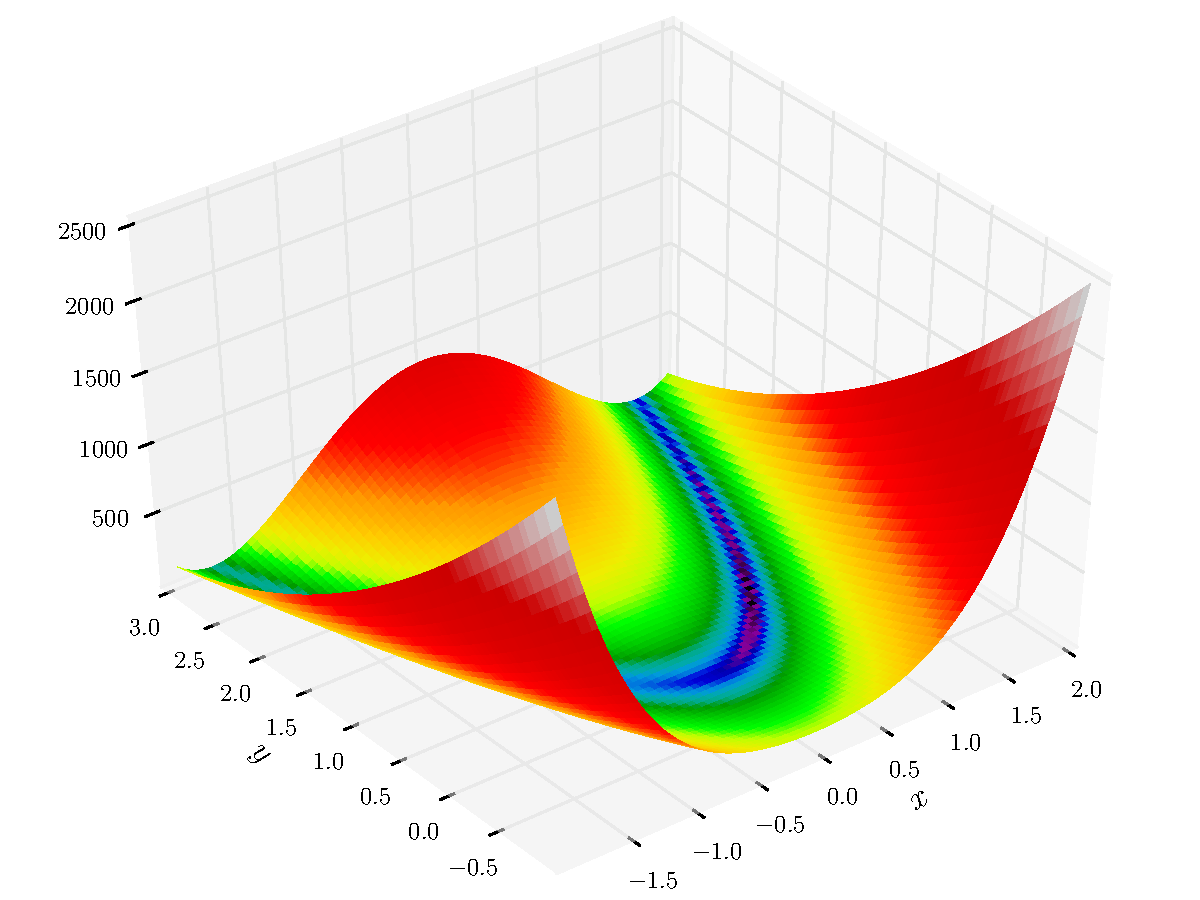
\includegraphics[width=0.6\textwidth]{rosenbrock.pdf}
    \caption{График функции Розенброка для двух переменных.}
    \label{rosenbrock_plot}
\end{figure}

\begin{table}
 \begin{tabular}{|*4{c|}}
\hline
\multicolumn{4}{|l|}{k = 1} \\
\hline
\multirow{1}{*}{\diagbox{$\mu$}{$\lambda$}} & \multicolumn{1}{c|}{1} & \multicolumn{1}{c|}{3} & \multicolumn{1}{c|}{7} \\
\hline
1 & 3631 & 2035 & 1226 \\
\hline
5 & 1666 & 1078 & 502 \\
\hline
10 & 1450 & 622 & 358 \\
\hline
\multicolumn{4}{|l|}{k = 2} \\
\hline
\multirow{1}{*}{\diagbox{$\mu$}{$\lambda$}} & \multicolumn{1}{c|}{1} & \multicolumn{1}{c|}{3} & \multicolumn{1}{c|}{7} \\
\hline
1 & 4744 & 1839 & 1160 \\
\hline
5 & 2467 & 1128 & 933 \\
\hline
10 & 1722 & 988 & 615 \\
\hline
\multicolumn{4}{|l|}{k = 3} \\
\hline
\multirow{1}{*}{\diagbox{$\mu$}{$\lambda$}} & \multicolumn{1}{c|}{1} & \multicolumn{1}{c|}{3} & \multicolumn{1}{c|}{7} \\
\hline
1 & 5159 & 2821 & 1517 \\
\hline
5 & 2704 & 1544 & 902 \\
\hline
10 & 2048 & 1296 & 1013 \\
\hline
\end{tabular}
\end{table}

\begin{table}
 \begin{tabular}{|*7{c|}}
\hline
\multicolumn{7}{|l|}{k = 1} \\
\hline
\multirow{2}{*}{\diagbox{$\mu$}{$\lambda$}} & \multicolumn{2}{c|}{1} & \multicolumn{2}{c|}{3} & \multicolumn{2}{c|}{7} \\
\cline{2-7}
 & q-learn & gecco & q-learn & gecco & q-learn & gecco \\
\hline
1 & 9653 & 8385 & 2226 & 1769 & 1105 & 1757 \\
\hline
5 & 1706 & 2281 & 894 & 942 & 570 & 675 \\
\hline
10 & 1103 & 1105 & 504 & 665 & 489 & 473 \\
\hline
\multicolumn{7}{|l|}{k = 2} \\
\hline
\multirow{2}{*}{\diagbox{$\mu$}{$\lambda$}} & \multicolumn{2}{c|}{1} & \multicolumn{2}{c|}{3} & \multicolumn{2}{c|}{7} \\
\cline{2-7}
 & q-learn & gecco & q-learn & gecco & q-learn & gecco \\
\hline
1 & 23663 & 21043 & 6405 & 6825 & 2388 & 2183 \\
\hline
5 & 3944 & 4029 & 1614 & 1780 & 1012 & 1461 \\
\hline
10 & 2108 & 2255 & 1420 & 1116 & 856 & 712 \\
\hline
\multicolumn{7}{|l|}{k = 3} \\
\hline
\multirow{2}{*}{\diagbox{$\mu$}{$\lambda$}} & \multicolumn{2}{c|}{1} & \multicolumn{2}{c|}{3} & \multicolumn{2}{c|}{7} \\
\cline{2-7}
 & q-learn & gecco & q-learn & gecco & q-learn & gecco \\
\hline
1 & 29082 & 23305 & 7977 & 10726 & 4680 & 4266 \\
\hline
5 & 6208 & 5419 & 2514 & 2096 & 1120 & 1629 \\
\hline
10 & 3747 & 3258 & 1740 & 1523 & 995 & 1203 \\
\hline
\end{tabular}
\end{table}

\begin{table}
 \begin{tabular}{|*7{c|}}
\hline
\multicolumn{7}{|l|}{k = 1} \\
\hline
\multirow{2}{*}{\diagbox{$\mu$}{$\lambda$}} & \multicolumn{2}{c|}{1} & \multicolumn{2}{c|}{3} & \multicolumn{2}{c|}{7} \\
\cline{2-7}
 & earpc & uearpc & earpc & uearpc & earpc & uearpc \\
\hline
1 & 7794 & 8689 & 3148 & 3610 & 1422 & 1422 \\
\hline
5 & 4341 & 4530 & 1958 & 2197 & 1679 & 1329 \\
\hline
10 & 2681 & 2926 & 1460 & 1485 & 1103 & 1858 \\
\hline
\multicolumn{7}{|l|}{k = 2} \\
\hline
\multirow{2}{*}{\diagbox{$\mu$}{$\lambda$}} & \multicolumn{2}{c|}{1} & \multicolumn{2}{c|}{3} & \multicolumn{2}{c|}{7} \\
\cline{2-7}
 & earpc & uearpc & earpc & uearpc & earpc & uearpc \\
\hline
1 & 27865 & 19142 & 9748 & 8997 & 3806 & 4085 \\
\hline
5 & 5961 & 5750 & 2293 & 1720 & 633 & 1180 \\
\hline
10 & 2411 & 2807 & 1486 & 1234 & 627 & 922 \\
\hline
\multicolumn{7}{|l|}{k = 3} \\
\hline
\multirow{2}{*}{\diagbox{$\mu$}{$\lambda$}} & \multicolumn{2}{c|}{1} & \multicolumn{2}{c|}{3} & \multicolumn{2}{c|}{7} \\
\cline{2-7}
 & earpc & uearpc & earpc & uearpc & earpc & uearpc \\
\hline
1 & 24249 & 27327 & 6541 & 16040 & 4144 & 5408 \\
\hline
5 & 5953 & 7665 & 2823 & 1304 & 1033 & 1055 \\
\hline
10 & 5095 & 3873 & 913 & 1028 & 679 & 839 \\
\hline
\end{tabular}
\end{table}

\section{Функция Леви}

Мультимодальная функция Леви для двух переменных задается формулой~(\ref{levi_eq}). График функции представлен на рис.~\ref{levi_plot}. При $x, y \in [-10; 10]$ минимум достигается в точке $(1, 1)$.

\begin{equation}
\label{levi_eq}
\begin{split}
f(x_1, x2) = &sin^2(3\pi x) + (x - 1)^2(1 + sin^2(3\pi y)) + \\
& + (y - 1)^2(1 + sin^2(2\pi y))
\end{split}
\end{equation}

\begin{figure}
    \centering
    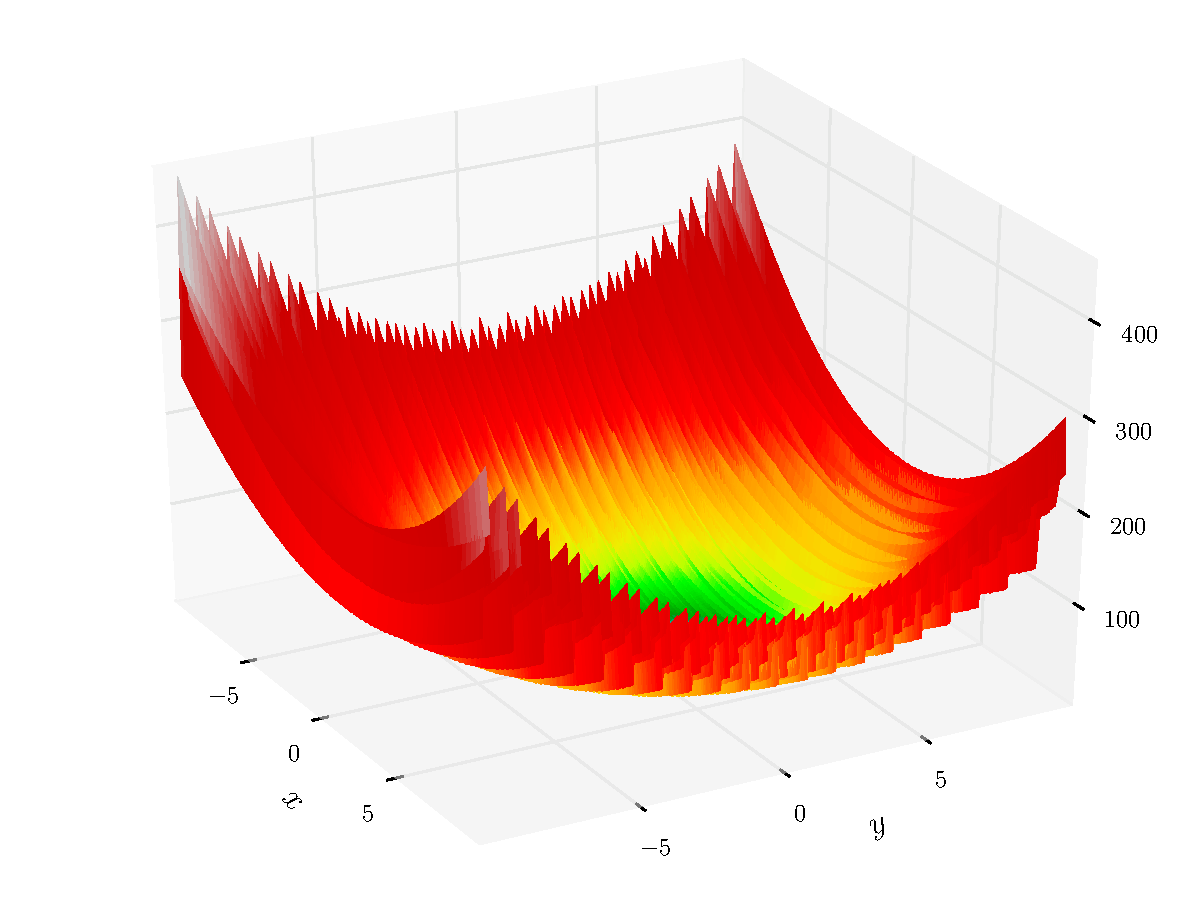
\includegraphics[width=0.6\textwidth]{levi.pdf}
    \caption{График функции Леви для двух переменных.}
    \label{levi_plot}
\end{figure}

\begin{table}
 \begin{tabular}{|*4{c|}}
\hline
\multicolumn{4}{|l|}{k = 1} \\
\hline
\multirow{1}{*}{\diagbox{$\mu$}{$\lambda$}} & \multicolumn{1}{c|}{1} & \multicolumn{1}{c|}{3} & \multicolumn{1}{c|}{7} \\
\hline
1 & 3496 & 1980 & 1321 \\
\hline
5 & 1778 & 855 & 504 \\
\hline
10 & 1305 & 717 & 456 \\
\hline
\multicolumn{4}{|l|}{k = 2} \\
\hline
\multirow{1}{*}{\diagbox{$\mu$}{$\lambda$}} & \multicolumn{1}{c|}{1} & \multicolumn{1}{c|}{3} & \multicolumn{1}{c|}{7} \\
\hline
1 & 4947 & 2020 & 1205 \\
\hline
5 & 1935 & 1085 & 953 \\
\hline
10 & 1803 & 918 & 801 \\
\hline
\multicolumn{4}{|l|}{k = 3} \\
\hline
\multirow{1}{*}{\diagbox{$\mu$}{$\lambda$}} & \multicolumn{1}{c|}{1} & \multicolumn{1}{c|}{3} & \multicolumn{1}{c|}{7} \\
\hline
1 & 5216 & 2900 & 1700 \\
\hline
5 & 3105 & 1808 & 1017 \\
\hline
10 & 2071 & 1330 & 904 \\
\hline
\end{tabular}
\end{table}

\begin{table}
 \begin{tabular}{|*7{c|}}
\hline
\multicolumn{7}{|l|}{k = 1} \\
\hline
\multirow{2}{*}{\diagbox{$\mu$}{$\lambda$}} & \multicolumn{2}{c|}{1} & \multicolumn{2}{c|}{3} & \multicolumn{2}{c|}{7} \\
\cline{2-7}
 & q-learn & gecco & q-learn & gecco & q-learn & gecco \\
\hline
1 & 7200 & 7265 & 3305 & 2903 & 1284 & 1600 \\
\hline
5 & 1898 & 1865 & 882 & 724 & 606 & 444 \\
\hline
10 & 840 & 764 & 502 & 624 & 331 & 294 \\
\hline
\multicolumn{7}{|l|}{k = 2} \\
\hline
\multirow{2}{*}{\diagbox{$\mu$}{$\lambda$}} & \multicolumn{2}{c|}{1} & \multicolumn{2}{c|}{3} & \multicolumn{2}{c|}{7} \\
\cline{2-7}
 & q-learn & gecco & q-learn & gecco & q-learn & gecco \\
\hline
1 & 13420 & 14789 & 6884 & 6601 & 3521 & 2370 \\
\hline
5 & 3517 & 3369 & 1031 & 1326 & 792 & 1089 \\
\hline
10 & 1884 & 2197 & 988 & 1006 & 731 & 564 \\
\hline
\multicolumn{7}{|l|}{k = 3} \\
\hline
\multirow{2}{*}{\diagbox{$\mu$}{$\lambda$}} & \multicolumn{2}{c|}{1} & \multicolumn{2}{c|}{3} & \multicolumn{2}{c|}{7} \\
\cline{2-7}
 & q-learn & gecco & q-learn & gecco & q-learn & gecco \\
\hline
1 & 21470 & 21953 & 9029 & 7071 & 4139 & 4019 \\
\hline
5 & 6966 & 6742 & 1467 & 2664 & 1929 & 1788 \\
\hline
10 & 2901 & 2943 & 1462 & 1832 & 1117 & 799 \\
\hline
\end{tabular}
\end{table}

\begin{table}
 \begin{tabular}{|*7{c|}}
\hline
\multicolumn{7}{|l|}{k = 1} \\
\hline
\multirow{2}{*}{\diagbox{$\mu$}{$\lambda$}} & \multicolumn{2}{c|}{1} & \multicolumn{2}{c|}{3} & \multicolumn{2}{c|}{7} \\
\cline{2-7}
 & earpc & uearpc & earpc & uearpc & earpc & uearpc \\
\hline
1 & 7986 & 14092 & 2789 & 3688 & 1923 & 3820 \\
\hline
5 & 2372 & 2246 & 1632 & 2171 & 1426 & 1236 \\
\hline
10 & 2353 & 1451 & 1491 & 1134 & 510 & 766 \\
\hline
\multicolumn{7}{|l|}{k = 2} \\
\hline
\multirow{2}{*}{\diagbox{$\mu$}{$\lambda$}} & \multicolumn{2}{c|}{1} & \multicolumn{2}{c|}{3} & \multicolumn{2}{c|}{7} \\
\cline{2-7}
 & earpc & uearpc & earpc & uearpc & earpc & uearpc \\
\hline
1 & 25721 & 30653 & 7477 & 4612 & 2533 & 2967 \\
\hline
5 & 7222 & 5365 & 3039 & 2943 & 1153 & 2180 \\
\hline
10 & 5139 & 3072 & 1045 & 2381 & 806 & 1064 \\
\hline
\multicolumn{7}{|l|}{k = 3} \\
\hline
\multirow{2}{*}{\diagbox{$\mu$}{$\lambda$}} & \multicolumn{2}{c|}{1} & \multicolumn{2}{c|}{3} & \multicolumn{2}{c|}{7} \\
\cline{2-7}
 & earpc & uearpc & earpc & uearpc & earpc & uearpc \\
\hline
1 & 28900 & 35119 & 6966 & 10883 & 3375 & 2062 \\
\hline
5 & 10480 & 9059 & 4593 & 3714 & 594 & 1439 \\
\hline
10 & 5210 & 4814 & 3140 & 2389 & 521 & 845 \\
\hline
\end{tabular}
\end{table}


\section{Функция Растригина}

Леонард Растригин предложил нелинейную мультимодальную функцию для тестирования эффективности алгоритмов оптимизации. Нахождение минимума этой функции затруднено большим количеством локальных минимумов в области поиска. Функция задается формулой~(\ref{rastrigin_eq}).

\begin{equation}
\label{rastrigin_eq}
f(x_1, .., x_n) = An + \sum\limits_{i = 1}^n\left[ x_i^2 - Acos\left(2 \pi x_i \right)\right]
\end{equation}

\subsection{Одномерный случай}

\begin{figure}
    \centering
    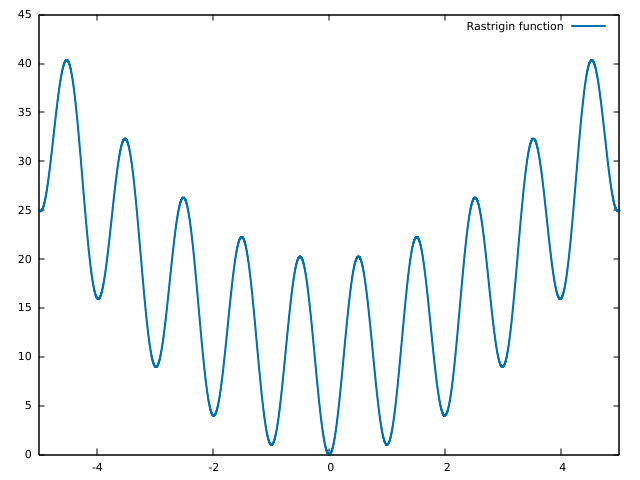
\includegraphics[width=0.6\textwidth]{rastrigin_1.png}
    \caption{График функции Растригина для одной переменной.}
    \label{rastrigin_plot}
\end{figure}

\begin{table}
 \begin{tabular}{|*4{c|}}
\hline
\multicolumn{4}{|l|}{k = 1} \\
\hline
\multirow{1}{*}{\diagbox{$\mu$}{$\lambda$}} & \multicolumn{1}{c|}{1} & \multicolumn{1}{c|}{3} & \multicolumn{1}{c|}{7} \\
\hline
1 & 734 & 273 & 147 \\
\hline
5 & 166 & 64 & 40 \\
\hline
10 & 93 & 56 & 22 \\
\hline
\multicolumn{4}{|l|}{k = 2} \\
\hline
\multirow{1}{*}{\diagbox{$\mu$}{$\lambda$}} & \multicolumn{1}{c|}{1} & \multicolumn{1}{c|}{3} & \multicolumn{1}{c|}{7} \\
\hline
1 & 767 & 409 & 167 \\
\hline
5 & 287 & 180 & 55 \\
\hline
10 & 167 & 65 & 45 \\
\hline
\multicolumn{4}{|l|}{k = 3} \\
\hline
\multirow{1}{*}{\diagbox{$\mu$}{$\lambda$}} & \multicolumn{1}{c|}{1} & \multicolumn{1}{c|}{3} & \multicolumn{1}{c|}{7} \\
\hline
1 & 889 & 579 & 282 \\
\hline
5 & 655 & 165 & 115 \\
\hline
10 & 247 & 98 & 38 \\
\hline
\end{tabular}
\end{table}

\begin{table}
 \begin{tabular}{|*7{c|}}
\hline
\multicolumn{7}{|l|}{k = 1} \\
\hline
\multirow{2}{*}{\diagbox{$\mu$}{$\lambda$}} & \multicolumn{2}{c|}{1} & \multicolumn{2}{c|}{3} & \multicolumn{2}{c|}{7} \\
\cline{2-7}
 & q-learn & gecco & q-learn & gecco & q-learn & gecco \\
\hline
1 & 994 & 767 & 331 & 329 & 133 & 224 \\
\hline
5 & 160 & 145 & 66 & 106 & 62 & 49 \\
\hline
10 & 111 & 109 & 53 & 34 & 31 & 31 \\
\hline
\multicolumn{7}{|l|}{k = 2} \\
\hline
\multirow{2}{*}{\diagbox{$\mu$}{$\lambda$}} & \multicolumn{2}{c|}{1} & \multicolumn{2}{c|}{3} & \multicolumn{2}{c|}{7} \\
\cline{2-7}
 & q-learn & gecco & q-learn & gecco & q-learn & gecco \\
\hline
1 & 1123 & 1018 & 318 & 449 & 192 & 221 \\
\hline
5 & 254 & 202 & 96 & 111 & 75 & 75 \\
\hline
10 & 101 & 83 & 43 & 106 & 47 & 41 \\
\hline
\multicolumn{7}{|l|}{k = 3} \\
\hline
\multirow{2}{*}{\diagbox{$\mu$}{$\lambda$}} & \multicolumn{2}{c|}{1} & \multicolumn{2}{c|}{3} & \multicolumn{2}{c|}{7} \\
\cline{2-7}
 & q-learn & gecco & q-learn & gecco & q-learn & gecco \\
\hline
1 & 2052 & 1258 & 400 & 957 & 245 & 255 \\
\hline
5 & 213 & 234 & 131 & 106 & 98 & 94 \\
\hline
10 & 114 & 190 & 109 & 82 & 65 & 28 \\
\hline
\end{tabular}
\end{table}

\begin{table}
 \begin{tabular}{|*7{c|}}
\hline
\multicolumn{7}{|l|}{k = 1} \\
\hline
\multirow{2}{*}{\diagbox{$\mu$}{$\lambda$}} & \multicolumn{2}{c|}{1} & \multicolumn{2}{c|}{3} & \multicolumn{2}{c|}{7} \\
\cline{2-7}
 & earpc & uearpc & earpc & uearpc & earpc & uearpc \\
\hline
1 & 382 & 694 & 378 & 367 & 146 & 171 \\
\hline
5 & 718 & 370 & 73 & 47 & 35 & 93 \\
\hline
10 & 104 & 52 & 36 & 32 & 22 & 18 \\
\hline
\multicolumn{7}{|l|}{k = 2} \\
\hline
\multirow{2}{*}{\diagbox{$\mu$}{$\lambda$}} & \multicolumn{2}{c|}{1} & \multicolumn{2}{c|}{3} & \multicolumn{2}{c|}{7} \\
\cline{2-7}
 & earpc & uearpc & earpc & uearpc & earpc & uearpc \\
\hline
1 & 1135 & 2793 & 243 & 256 & 393 & 250 \\
\hline
5 & 379 & 337 & 110 & 259 & 35 & 77 \\
\hline
10 & 85 & 313 & 134 & 80 & 23 & 20 \\
\hline
\multicolumn{7}{|l|}{k = 3} \\
\hline
\multirow{2}{*}{\diagbox{$\mu$}{$\lambda$}} & \multicolumn{2}{c|}{1} & \multicolumn{2}{c|}{3} & \multicolumn{2}{c|}{7} \\
\cline{2-7}
 & earpc & uearpc & earpc & uearpc & earpc & uearpc \\
\hline
1 & 1712 & 2735 & 653 & 289 & 346 & 537 \\
\hline
5 & 827 & 313 & 138 & 158 & 88 & 59 \\
\hline
10 & 478 & 169 & 36 & 59 & 30 & 68 \\
\hline
\end{tabular}
\end{table}


\subsection{Двумерный случай}

\begin{figure}
    \centering
    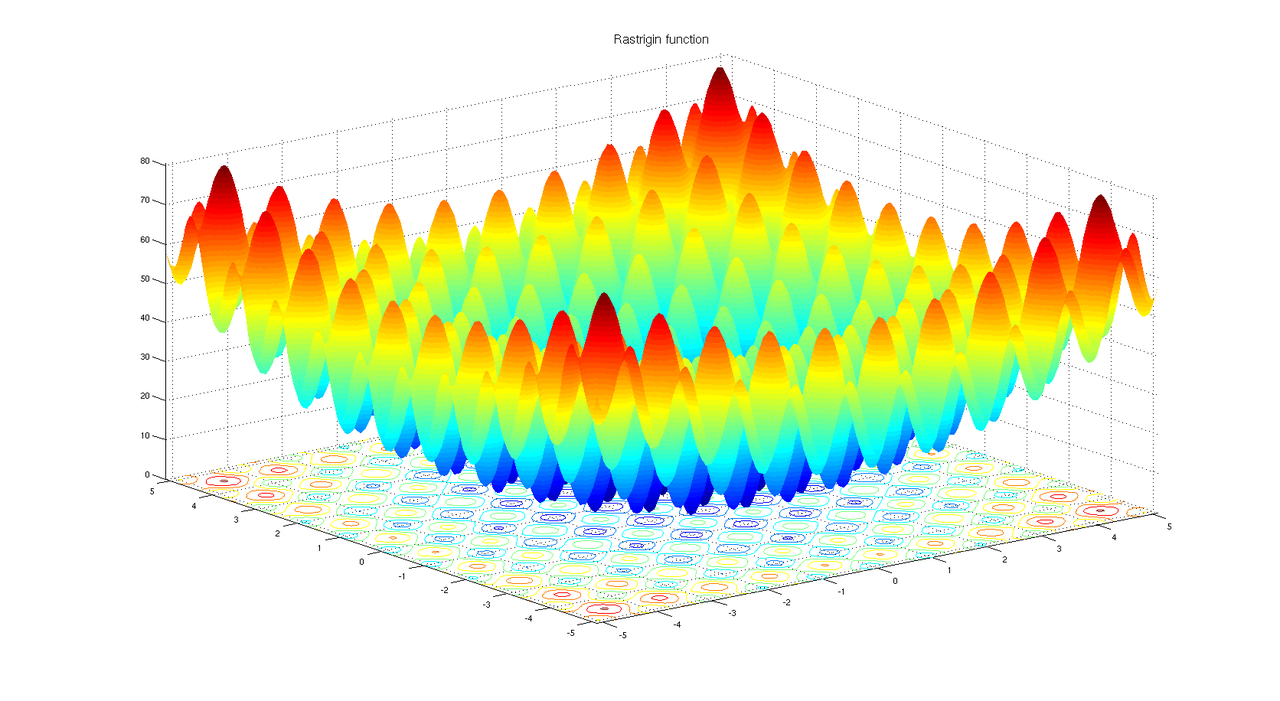
\includegraphics[width=0.6\textwidth]{rastrigin_2.png}
    \caption{График функции Растригина для двух переменных.}
    \label{rastrigin_plot}
\end{figure}

\begin{table}
 \begin{tabular}{|*4{c|}}
\hline
\multicolumn{4}{|l|}{k = 1} \\
\hline
\multirow{1}{*}{\diagbox{$\mu$}{$\lambda$}} & \multicolumn{1}{c|}{1} & \multicolumn{1}{c|}{3} & \multicolumn{1}{c|}{7} \\
\hline
1 & 5124 & 2301 & 1411 \\
\hline
5 & 1859 & 1053 & 988 \\
\hline
10 & 1617 & 1157 & 865 \\
\hline
\multicolumn{4}{|l|}{k = 2} \\
\hline
\multirow{1}{*}{\diagbox{$\mu$}{$\lambda$}} & \multicolumn{1}{c|}{1} & \multicolumn{1}{c|}{3} & \multicolumn{1}{c|}{7} \\
\hline
1 & 5165 & 3461 & 1753 \\
\hline
5 & 1990 & 1396 & 1095 \\
\hline
10 & 2022 & 1354 & 998 \\
\hline
\multicolumn{4}{|l|}{k = 3} \\
\hline
\multirow{1}{*}{\diagbox{$\mu$}{$\lambda$}} & \multicolumn{1}{c|}{1} & \multicolumn{1}{c|}{3} & \multicolumn{1}{c|}{7} \\
\hline
1 & 6535 & 3391 & 2573 \\
\hline
5 & 3148 & 1721 & 1231 \\
\hline
10 & 2352 & 1677 & 1119 \\
\hline
\end{tabular}
\end{table}


\begin{table}
 \begin{tabular}{|*7{c|}}
\hline
\multicolumn{7}{|l|}{k = 1} \\
\hline
\multirow{2}{*}{\diagbox{$\mu$}{$\lambda$}} & \multicolumn{2}{c|}{1} & \multicolumn{2}{c|}{3} & \multicolumn{2}{c|}{7} \\
\cline{2-7}
 & q-learn & gecco & q-learn & gecco & q-learn & gecco \\
\hline
1 & 15058 & 13418 & 3914 & 4167 & 1791 & 2330 \\
\hline
5 & 2311 & 2809 & 869 & 748 & 533 & 665 \\
\hline
10 & 1497 & 1593 & 488 & 616 & 290 & 235 \\
\hline
\multicolumn{7}{|l|}{k = 2} \\
\hline
\multirow{2}{*}{\diagbox{$\mu$}{$\lambda$}} & \multicolumn{2}{c|}{1} & \multicolumn{2}{c|}{3} & \multicolumn{2}{c|}{7} \\
\cline{2-7}
 & q-learn & gecco & q-learn & gecco & q-learn & gecco \\
\hline
1 & 23371 & 27239 & 7295 & 7169 & 3488 & 2968 \\
\hline
5 & 8076 & 5810 & 2116 & 2705 & 1001 & 1247 \\
\hline
10 & 3415 & 2787 & 1037 & 1106 & 811 & 666 \\
\hline
\multicolumn{7}{|l|}{k = 3} \\
\hline
\multirow{2}{*}{\diagbox{$\mu$}{$\lambda$}} & \multicolumn{2}{c|}{1} & \multicolumn{2}{c|}{3} & \multicolumn{2}{c|}{7} \\
\cline{2-7}
 & q-learn & gecco & q-learn & gecco & q-learn & gecco \\
\hline
1 & 28702 & 36597 & 11427 & 9873 & 5820 & 6462 \\
\hline
5 & 12438 & 6791 & 2289 & 3673 & 1626 & 1255 \\
\hline
10 & 4473 & 6531 & 2000 & 1650 & 1137 & 1098 \\
\hline
\end{tabular}
\end{table}

\begin{table}
 \begin{tabular}{|*7{c|}}
\hline
\multicolumn{7}{|l|}{k = 1} \\
\hline
\multirow{2}{*}{\diagbox{$\mu$}{$\lambda$}} & \multicolumn{2}{c|}{1} & \multicolumn{2}{c|}{3} & \multicolumn{2}{c|}{7} \\
\cline{2-7}
 & earpc & uearpc & earpc & uearpc & earpc & uearpc \\
\hline
1 & 9003 & 12905 & 3553 & 1701 & 2296 & 1941 \\
\hline
5 & 5730 & 4453 & 1393 & 2749 & 1130 & 1258 \\
\hline
10 & 2213 & 3085 & 1161 & 1225 & 391 & 429 \\
\hline
\multicolumn{7}{|l|}{k = 2} \\
\hline
\multirow{2}{*}{\diagbox{$\mu$}{$\lambda$}} & \multicolumn{2}{c|}{1} & \multicolumn{2}{c|}{3} & \multicolumn{2}{c|}{7} \\
\cline{2-7}
 & earpc & uearpc & earpc & uearpc & earpc & uearpc \\
\hline
1 & 20005 & 20819 & 7166 & 13342 & 5874 & 7870 \\
\hline
5 & 11153 & 11856 & 3775 & 4542 & 1775 & 2584 \\
\hline
10 & 8768 & 4603 & 3719 & 1648 & 1740 & 2558 \\
\hline
\multicolumn{7}{|l|}{k = 3} \\
\hline
\multirow{2}{*}{\diagbox{$\mu$}{$\lambda$}} & \multicolumn{2}{c|}{1} & \multicolumn{2}{c|}{3} & \multicolumn{2}{c|}{7} \\
\cline{2-7}
 & earpc & uearpc & earpc & uearpc & earpc & uearpc \\
\hline
1 & 32533 & 43832 & 13061 & 10068 & 9797 & 9775 \\
\hline
5 & 8320 & 10539 & 4434 & 6799 & 2951 & 4914 \\
\hline
10 & 8952 & 11581 & 2611 & 1307 & 1742 & 2479 \\
\hline
\end{tabular}
\end{table}


\section{Выводы}
